\newpage
\section{Process Environment}


% Kill di un processo in C
\subsection{Kill di un processo in C}

Per far \hl{terminare un processo} usiamo:

\begin{enumerate}
    \item \hl{return} dal main
    \item chiamando \hl{exit}: \textbf{chiudo la singola thread} ma poi passa da un \textbf{gestore di exit (exit function)} che chiama gli \txtbf{exit handler} che possono essere installati e aggiunti tramite la funzione
\begin{lstlisting}
int atexit(void (*func)(void));
\end{lstlisting}
    e verranno richiamate in ordine contrario alla dichiarazione
    
    \item chiamando \hl{\_exit o \_Exit}: usate per terminare il processo e \textbf{finire direttamente nel kernel} senza passare dall'exit function
    \item \hl{return dell'ultima thread}
    \item chiando \hl{pthread\_exit dall'ultima thread}
    \item chiamando \hl{abort}: che \textbf{genera un segnale gestibile SIGABRT}, ma che fa comunque teminare il processo
    \item ricevendo un \hl{segnale}: come \textbf{SIGKILL e SIGSTOP} che non potranno essere gestiti o fermati
    \item \hl{richiesta di cancellazione} dell'ultima thread
\end{enumerate}


% Environment list
\subsection{Environment list}

Quando si va a \hl{creare una variabile} nello schell:

\begin{lstlisting}
$ a=100
\end{lstlisting}

questa \hl{non viene passara al child schell}, come "env", a meno di non \hl{usare il builtin "export"}.

In un processo \hl{possiamo vedere le variabli di ambiente in runtime}, tramite il debugger, ma non nello stesso punto in cui si trovano. \hl{Per le variabili di ambiente} abbiamo che:


\begin{figure}[H]
\centering
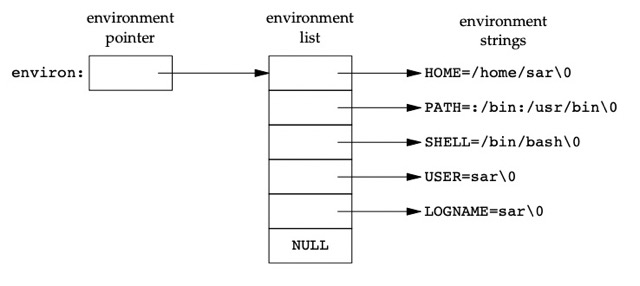
\includegraphics[scale=0.4]{varamb.jpeg}
\caption{Variabili di ambiente} 
\label{varamb}
\end{figure}


dove ogni valore è \hl{separato da un null $\backslash 0$} e \hl{storicizzato in un array di puntatori} andando a terminare con un null.

I programmi, tramite un \hl{handle}, possono \hl{accedere a questo array tramite un altro puntatore} (environment pointer), come:

\begin{lstlisting}
extern char **environ;
\end{lstlisting}

oppure nel \hl{main}:
\begin{lstlisting}
int main(int argc, char *argv[], char *envp[]);
\end{lstlisting}

oppure con la \hl{funzione}:
\begin{lstlisting}
char *getenv(const char *name);
\end{lstlisting}

che \hl{passando il nome della variaible di ambiente restituendo un puntatore al suo contenuto}.

Notare che la \hl{malloc usa zone globali allora non è rientrant}, vedremo poi cosa vuol dire.






(VEDERE memory\_dump.c) che vede e sampa tutte le variabili di mabinete, aspetta un p`o e poi lo ri fa stampandone anche di nuove e modificandone una esistente e poi va a vedere rispetto ai punttori precendenti c se sno ancora buoni  o se stanno da un altra parte

vedere a mush simpler way to print addresses used in process memory per stampare semplicemtne gli indirizzi delle variabili di ambiente


in memory\_dump.c abbiamo un popen che restituisce un puntatore di tipo file che e1 uin ingresso alla pipe [in pratica ]

con sort -n ordine numerico -r reverce -k3 chiave (colonna) da scegliere con w dico che la triga la vogli scrivere nella pipe

notiamo che le libreire di namiche stanno da tutaltra parte delle funzioni che osno del programma che sono come puntatori al text (stano in basso)
infatti vediamo con $(()) che abbimao 216 byte tra i puntato di envp0 e envp27 con $(()) notiamo che abbiamo solo 64 bit a sisposizione id cui uno e1 per il segno in quel caso usiamo bc

il programma vuole capire cosa succedere alle variabilei di imabiente quando vanno modificate o agiunte

putenv: mette direttamente dove sono le variabili di ambiente prende una tringa cheha tutta la variabile di ambiente: name=value e se c'e1 gia1 non fa nulla
setenv: si appoggia di una memoria alllocata

negli if crea delle variabili con putenv e vuole andare a vedre dove sono

display var ambient:
loop sulle variabili di ambiente e setta "\&" poi in strncopy copia un buf+1 la stringa della varaibile prendendo size buf-2 perche togliamo $\backslash 0$ e \&
per printare fa un mkPrintable per evitare di avere strani segni nell'output
dumpAddr() fa una fprintf nel puntatore per dargli la riga da sptampre



una pipe e1 una struttura con ...

dato che popen onn e1 sicura faccio la chiamata pipe una fork e poi il chil una exec del sort


strchr: isola in nome della variaible e poi nell'if vede se il nome e1 TERM, se TERM e1 definita e verifca se il puntatore vero e1 diverso da quello nuovo e quindi vede se la variabil e1 stat cambiata
allora aggancia a TERM @ e = e poi aggiunge l'ltimo agiornamtne della varaibile di ambiente (quella cambiata) 
con cp che indica dove e1 stata spostata la varaibile

qindi le nuove varaibili modificate sanno inun tunto della memoria diverso da quello iniziale dato che in genre son incastarete tra loro tramite un unica stringa ma separate da un \0 allora si e1 pensato di carearne direttamente un altra in un altro punto di memoria e la get env si preoccupa di fare tutto e di dire che non si deve piu fare affidamente al vecchio puntatore alla variabile ma al nuovo

ricordare che 
gli standard fanno rispettare le interfaccie e non le implementazioni quindi fanno rispettare parametri e return della funzione ma non cosa fa dentro

per vedere le aree di memoria per le quali il porcesso ha il permesso:
vmmap -resident ointerleaved 9163

su linux 
cat /proc/$$/maps


setjump e longjump:

serve quando hai tanti stack frame che hanno fatto elaborazioni lunghe e lo stack siallunga, allora nell'ultima chiamata potremmo volr uscre e rifare il corcorso al contratrio per chiuderela tendina degli stack frame allora quando dienta lunga puo esser comodo dire di togliere tutti li stack frame e andare direttametn allinizio. fiunziona con le chiamate setjump e longjump
1. la fa nella funzione chiamante nela qule si vuole fare il return per esmpio di puo ritorna alla prima, eliminando tutti le azioni intermedie perche no nci soddisfa un valore e vlgiamo rincomunicare da zero. allora si passa al setjump una fotografica del tipo della variabile jmp\_buf env. questa prima chiamata fa return di zero per dirti che la foto della varaibiel sta storizzata bene. se poi volgiamo ritornare allinizion tramite longjumop si ritorna setjump passandogli la fotografi jmp\_buf env e anceh un int val che rappresenta, come se avessi fatto la setjump solo che gil fa ritornare la variabile val impostando il valore del return della setjump. dato che puoessere chiamata da tanti posti al longjump allora ritorna un numero diverso in base a dove si trovano